\subsubsection{Setting up Environment variables}

\paragraph{AWS environment variables}
To setup the AWS environment variables, open the AWS Management Console (\url{https://aws.amazon.com/it/console/}) and, in the search bar search 'Parameter Store' and click on the 'Systes Manager Parameter Store' feature.

From there, the following parameters are needed:

\begin{itemize}
\item STRIPE\textunderscore KEY\textunderscore \$STAGE: the Stripe private API key you can find on the stripe website, in the API keys page. You must create one parameter for each of your stages;
\item STRIPE\textunderscore SIGN\textunderscore \$STAGE: the Stripe signing key you can find on the stripe website, in the Webhooks page. You must create one parameter for each of your stages;
\item EMAIL: the email address used to send the confirmation email after a purchase;
\item PASS\textunderscore EMAIL: the password to the email address used to send the confirmation email after a purchase.
\end{itemize}
 
After setting up the AWS Parameters, redeploy the back-end module as shown previously in section §3.3.2

\paragraph{Vercel environment variables}
\begin{enumerate}
\item login into vercel website, click on the project you created and go to "Settings". Now go on "Environment Variables". Here you can set the environment variables needed for the project.\\
\begin{figure}[H]
\centering
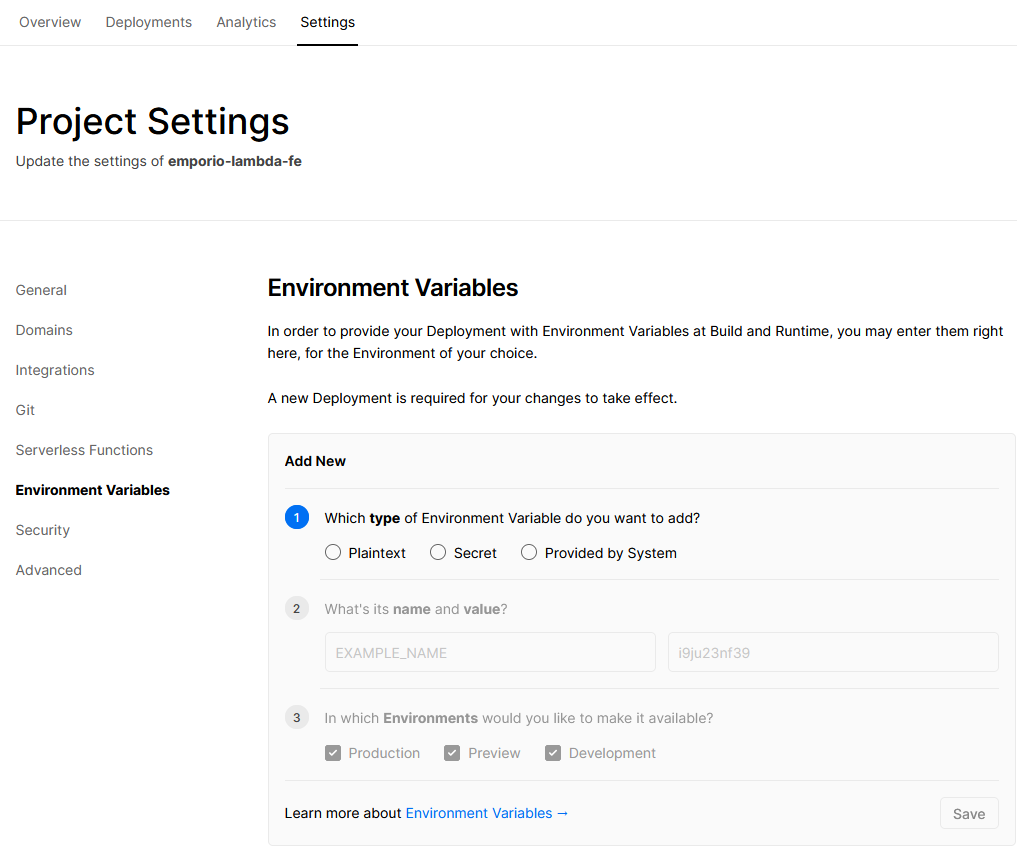
\includegraphics[scale=0.55]{res/Setup/Configurazione/img/settingsEnvVar}\\
\caption{Example of the vercel website UI}
\end{figure}
The following environment variables are needed:\\
\setcounter{table}{-1}
{
\rowcolors{2}{azzurro2}{azzurro3}
\centering
\renewcommand{\arraystretch}{1.5}
\begin{longtable}{c C{6cm} C{3cm} C{5cm}}
\rowcolor{azzurro1}
\textbf{Type} &
\textbf{Name} &
\textbf{Environment} &
\textbf{How to get/Value}\\
\endhead

Plaintext & NEXT\_PUBLIC\_STRIPE & Production, Preview, Development & Informations on how to get this variable can be found here \url{https://stripe.com/docs/keys}\\
Plaintext & NEXTAUTH\_URL & Production & Set it as your Production domain in Vercel\textsubscript{G}.\\
Plaintext & COGNITO\_LOGOUT\_URL & Production & Set it as your production domain in Vercel\textsubscript{G}.\\
Plaintext & COGNITO\_DOMAIN & Production & Insert here the AWS Cognito domain you use for the Production stage.\\
Plaintext & COGNITO\_CLIENT\_ID & Production & Insert here the ID of the AWS Cognito User Pool you use for the Production stage.\\
Plaintext & NEXTAUTH\_URL & Preview & Insert here the domain you use for the Preview stage.\\
Plaintext & COGNITO\_LOGOUT\_URL & Preview & Insert here the domain you use for the Preview stage.\\
Plaintext & COGNITO\_DOMAIN & Preview & Insert here the AWS Cognito domain you use for the Preview stage.\\
Plaintext & COGNITO\_CLIENT\_ID & Preview & Insert here the ID of the AWS Cognito User Pool you use for the Preview stage.\\
Plaintext & NEXTAUTH\_URL & Development & http://localhost:3000 \\
Plaintext & COGNITO\_LOGOUT\_URL & Development & http://localhost:3000 \\
Plaintext & COGNITO\_DOMAIN & Development & Insert here the AWS Cognito User Pool domain you use for the Development stage.\\
Plaintext & COGNITO\_CLIENT\_ID & Development & Insert here the ID of the AWS Cognito User Pool you use for the local stage.\\
Plaintext & NEXT\_PUBLIC\_SITE & Production & Insert here the Domain of the website for the Production stage.\\
Plaintext & NEXT\_PUBLIC\_SITE & Preview & Insert here the Domain of the website for the Preview stage.\\
Plaintext & NEXT\_PUBLIC\_SITE & Development & http://localhost:3000\\
Plaintext & NEXT\_PUBLIC\_STAGE & Production & staging\\
Plaintext & NEXT\_PUBLIC\_STAGE & Preview & test\\
Plaintext & NEXT\_PUBLIC\_STAGE & Development & local\\
Secret & NEXT\_PUBLIC\_API\_ID & Production & API endpoint id provided by AWS when the backend is deployed to the staging environment (or the domain, if used)\\
Plaintext & NEXT\_PUBLIC\_API\_ID & Preview & API endpoint id provided by AWS when the backend is deployed to the test environment (or the domain, if used)\\
Plaintext & NEXT\_PUBLIC\_API\_ID & Development & API endpoint id provided by AWS when he backend is deployed to the local environment (or the domain, if used)\\
Plaintext & NEXT\_PUBLIC\_REGION\_API & Production, Preview, Development & Insert here the location of your AWS account (example: eu-central-1) \\
Plaintext & NEXT\_PUBLIC\_API\_PROTOCOL & Production, Preview, Development & https \\
Plaintext & NEXT\_PUBLIC\_API\_DOMAIN & Production, Preview, Development & amazonaws.com \\
Plaintext & NEXT\_PUBLIC\_API\_SERVICE & Production, Preview, Development & execute-api \\
Plaintext & JWT\_SIGNING\_PRIVATE\_KEY & Production, Preview, Development & run the commands:
\begin{enumerate}
\item \texttt{npm i -g node-jose-tools;}
\item \texttt{jose newkey -s 512 -t oct -a HS512;}
\item the output is the value you need.
\end{enumerate}\\
\end{longtable}
}

\item in your CLI use the command\begin{center}\texttt{vercel env pull}\end{center} This will download and setup your environment variables.
\end{enumerate}

\paragraph{Github environment variables}
If you're using github as a git repository you can also use the provided Github actions workflows to automatically deploy you back-end and front-end on each push. To do so you need to set up a few github secrets:
\begin{itemize}
\item Front-end module:	the required secrets can be found on this page \url{https://github.com/marketplace/actions/vercel-action};
\item Back-end module: the two required secrets are:
\begin{itemize}
\item AWS\_ACCESS\_KEY\_ID
\item AWS\_SECRET\_ACCESS\_KEY
\end{itemize}
which are the same keys used for the serverless setup, described in section §3.3.2.
\end{itemize}